\section{Free laser drift analysis}\label{freedrift}
\subsection{Free evolution}
To study how the evolution worked we acquired some measurements of the laser output using the spectrometer and the etalon, while keeping constant all the laser parameters (current, temperature and piezoelectric voltage). At first we took a short term measurement lasting 20 minutes. But we understood that the evolution was quite slow, and that this first measurement was too short to be meaningful. We then took a second long term measurement, lasting a night time, in order to see whether a stable regime was reached. These are shown in \cref{senzaniente}.

The first thing we noticed was that the mode hopping due to the uncontrolled evolution followed the same pattern as the mode hopping due to the piezoelectric movement (see an example in \cref{hoppattern,tabrutta}). This suggested us the idea that one of the factors which generating this evolution could be a movement of the grating of the ECDL, allegedly caused by thermal expansion of the cage system holding it. 

\begin{figure}[!hptb]\centering
\subfigure[Twenty minutes measurement. No equilibrium configuration is reached, nor clear pattern is visible. Laser parameters: 29,50 $^\circ$C; 80,00 mA.\label{senzaniente20}]{\includegraphics[width=\linewidth, height=9.5cm, draft=\foto]{eps/20minuteshops.eps}} 
\subfigure[Twelve hours measurement. A low frequency pattern appears, and this looks very similar to the mode hopping pattern due to the grating movements. Laser parameters: 25,03 $^\circ$C; 80,01 mA.\label{senzaniente12h}]{\includegraphics[width=\linewidth, height=9.5cm, draft=\foto]{eps/nighttime.eps}}
\caption{Laser free drift measurements.}
\label{senzaniente}
\end{figure} 
 
\subsection{Heating- and cooling-induced evolution}

In order to confirm the fact that the evolution depends mainly on temperature (of the cage system or of the air) effects we put a tungsten lamp near the ECDL and turned it on. As we can see from \cref{lampdrift}, turning on the lamp increased the speed of the evolution a lot. After keeping the lamp on for a while we turned it off and took another measurement. This time we observed an evolution pattern almost as fast as the one with the lamp on, but with a reverse pattern. We interpreted this a signal that the system is cooling down.

\begin{figure}[!t]\centering
\includegraphics[width=\linewidth, draft=\foto]{eps/lampandnot.eps}
\caption{During the measurements with the lamp turned on we were  eventually able to see the difference in the minimum and maximum wavelength of the same mode after some drifts, as represented in the next graphic. Laser parameters: 27,68\cel; 80,01  mA.}
\label{lampdrift}
\end{figure}

\begin{figure}[!b]\centering
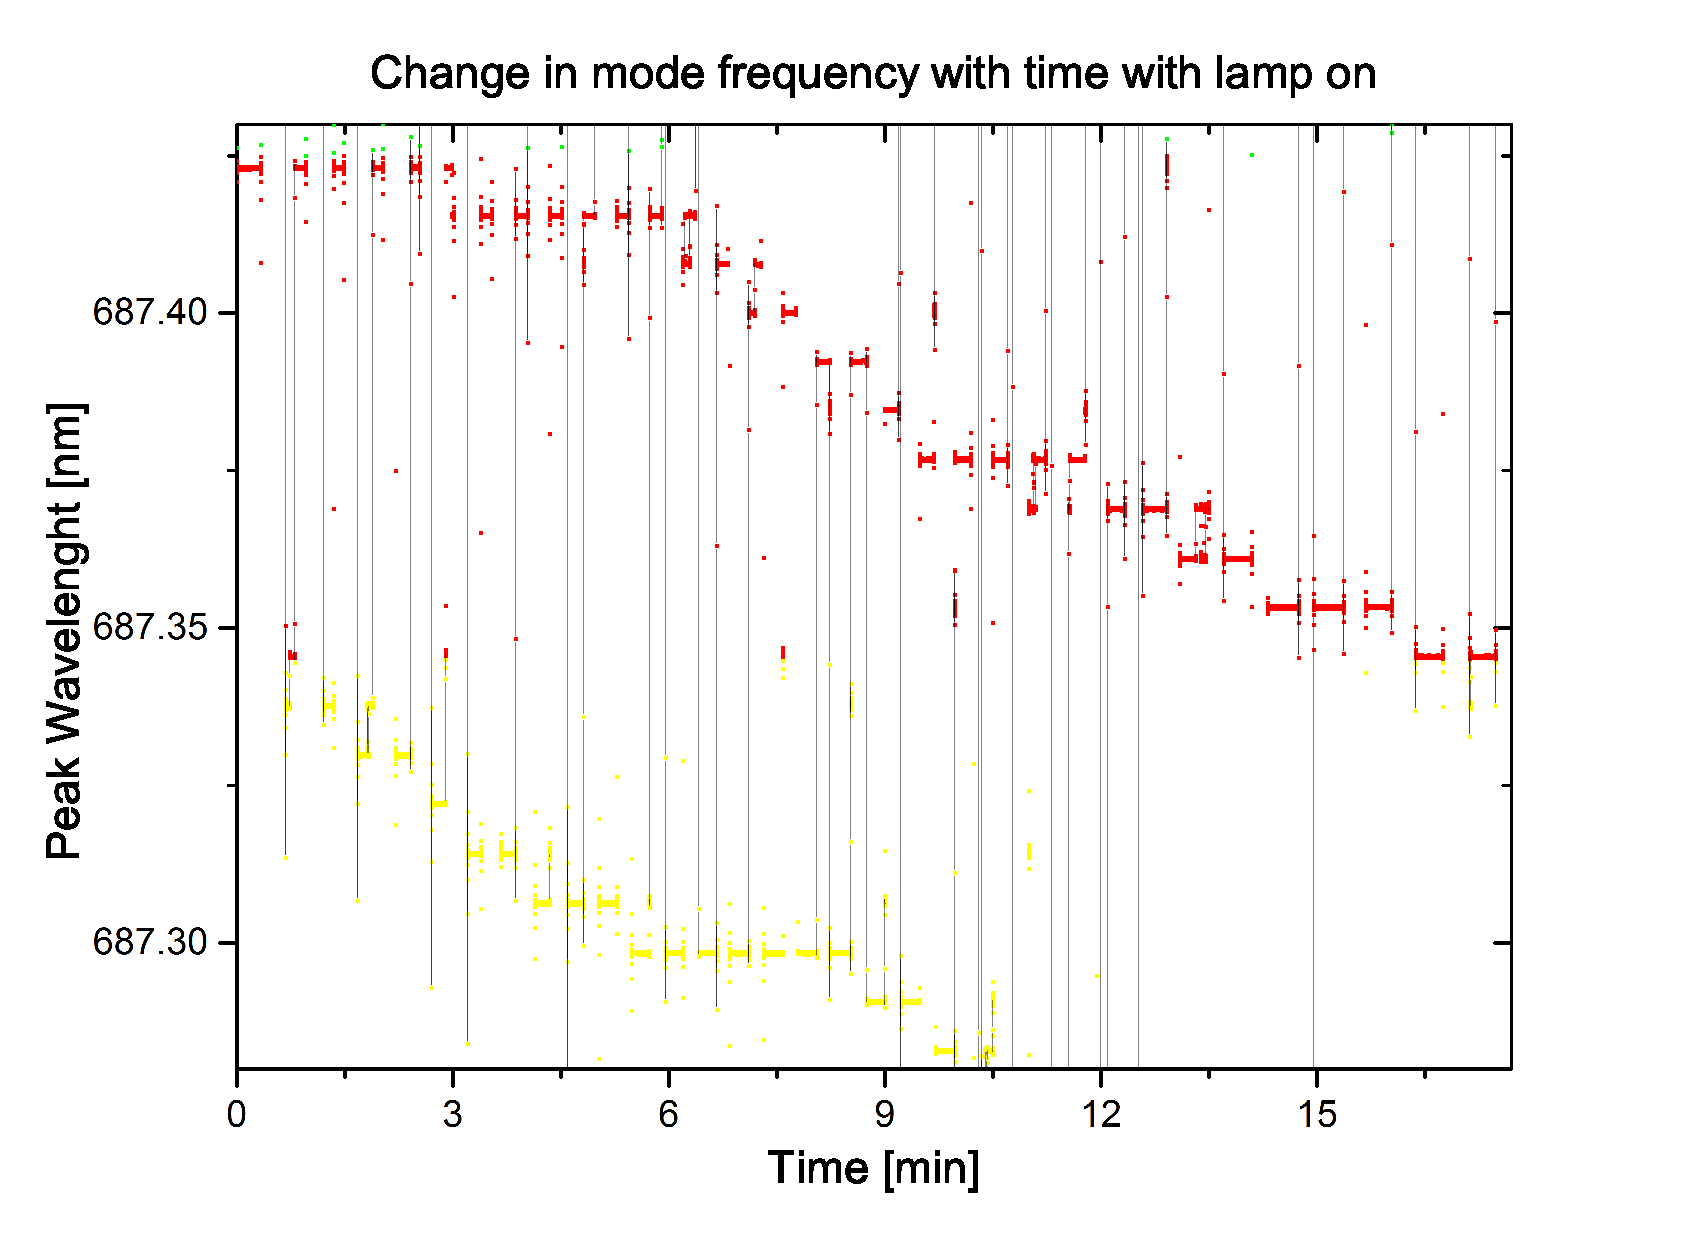
\includegraphics[width=\linewidth, draft=\foto]{eps/modedrift.eps}
\caption{The wavelength of both of the mode shown here decreases after some periods of hopping. Laser parameters: 25.03\cel; 80.01 mA.}
\label{modedrift}
\end{figure}
 
\subsection{Tunability change measurement}
Since the resolution of our spectrometer was usually not good enough to distinguish a tunability change in time, we used the etalon to take a measurement similar to the tunability measurement of a mode (687.45 nm) several times, measuring the minimum  and maximum wavelength before a mode hop for about two hours.
The results in \cref{minmaxshift} show how not only the minimum and maximum piezoelectric voltages, but also the position of the etalon interference pattern change in time. Considering that the etalon FSR is of the order of 3-4 microseconds (on the video camera PAL signal), we found that the min-max drift is of the order of about one half as the tunability found in \cref{tuna}.
%is of the order of the Ghz/timeunitnoncostante
%l'incertità dei dati dovuta alla larghezza dei picchi (che conta un tot) nella tabella è dei soliti 40ns/2radq2log2 cioè di circsa 2.12330450072005E-007 s ma forse un po' menosispera. l'errore di risoluz dell'oscillocoso sarebbe invece 40 ns /radq12).
\begin{table}[!p]
\begin{tabular}{|c|c|c|c|c|c|}
\hline
Time [min] & $\Delta$Min [ns] & Min volt. [V] & $\Delta$Max [ns] & Max volt. [V] & Tunab. [ns] \\ \hline
%0 & 9.677 & 3 & 9.678 & 17 & 560 \\ \hline
15 & 0 & 19 & 180 & 24 & 720 \\ \hline
30 & 250 & 20 & $<$40 & 27 & 500 \\ \hline
50 & 260 & 23 & 260 & 29 & 480 \\ \hline
95 & -330 & 23 & -360 & 29 & 440 \\ \hline
135 & 330 & 29 & 220 & 38 & 560 \\ \hline
\end{tabular}
\caption{Shifts of the maximum and minimum positions on the oscilloscope of the 687.45 nm mode. As discussed in \cref{tuna}, the uncertainty on the time measurement is estimated to be $\simeq$ 40 ns.}
\label{minmaxshift}
\end{table}